\documentclass[nofonts]{ctexart}
%\CTEXsetup[name={Step ,},number={\arabic{chapter}}]{chapter}

\setCJKmainfont[ItalicFont={AR PL UKai CN}]{AR PL UMing CN} %设置中文默认字体
\setCJKsansfont{WenQuanYi Micro Hei} %设置文泉驿正黑字体作为中文无衬线字体
\setCJKmonofont{WenQuanYi Micro Hei Mono} %设置文泉驿等宽正黑字体作为中文打字机字体

\usepackage{amsmath}
%\usepackage{wallpaper}
\usepackage{xcolor}
%\usepackage{pgf, tikz}
\usepackage{multirow}
\usepackage{listings}
\usepackage{color}

\definecolor{keywordcolor}{rgb}{0.8,0.1,0.5}
\definecolor{webgreen}{rgb}{0,.5,0}

%\usepackage[paperwidth=185mm,paperheight=260mm,text={148mm,210mm},left=21mm,includehead,vmarginratio=1:1]{geometry}
%\usepackage[raggedright]{titlesec}
%\titleformat{\chapter}[display]{\Huge\bfseries}{Step \,\thechapter\,}{1em}{}

%\usepackage{fancyhdr}
%\pagestyle{fancy}
%\fancyhf{}
%\fancyhead[ER, OR]{\leftmark}
%\fancyhead[EL, OL]{《编译实习》实习报告}
%\fancyfoot[C]{\thepage}
%\renewcommand{\chaptermark}[1]{\markboth{\thechapter.\ #1}{}}


\lstset{language=C,
basicstyle=\footnotesize,
keywordstyle=\color{keywordcolor}\bfseries, %\underbar,
identifierstyle=,
commentstyle=\color{green} \textit,
stringstyle=\color{red} \ttfamily,
showstringspaces=false,
frame=single,
numbers=left,
numberstyle=\tiny \color{blue},
backgroundcolor=\color{white},
captionpos=b
}


\begin{document}

\title{%
\vspace{-30mm}\Huge NachOS Lab2 实习报告 \vspace{10mm}}
\author{%
\Large 史杨勍惟 
\\[10mm] 1200012741 信息科学技术学院}
\date{2016,04,12}

\maketitle

\newpage
\tableofcontents
\newpage

\section{总体概述}
这次lab的主要内容在于对nachos现有调度算法的深入理解和扩展。工作量相对于上次的lab多了一些。而工作内容则更偏向于底层。
这次lab另一个特点是灵活,由于Challenge的存在,所以后面的设计是开放性的。不过也需要我们对调度算法有个更深入的理解。
我在Nachos中整合了四个不同的调度算法,分别是原始的FIFO,以及新增的基于优先级的抢占式,RR算法,和一个简单的类似Linux的调度算法。


\section{任务完成列表}
\begin{table}[h]
\centering
\footnotesize
\begin{tabular}{|c|c|c|c|}\hline
\textbf{Exercise 1} & \textbf{Exercise 2} & \textbf{Exercise 3} & \textbf{Challenge 1} \\\hline
Y & Y & Y & Y \\\hline

\end{tabular}

\end{table}
\section{完成情况}
\subsection*{Exercise 1}
\textbf{调研Linux或Windows中采用的进程调度算法}\\
我主要调研的是Linux的进程调度算法,因为在我的实现中加入了简单的类似Linux的调度算法。Linux的调度算法为CFS算法,其主要设计思想是:

Linux把所有要调度的进程在一个进程周期先后调度上。把进程的优先级看成两个不同的维度,一个是这个进程在单位调度周期中运行的时间,另一个则是这个进程在这个调度周期中被分配上CPU的顺序。其中,
\begin{itemize}
\item 执行时间由进程的给定nice值决定。
\item 执行的先后由这个进程已运行的虚拟运行时间决定,这个虚拟运行时间差不多为实际运行时间除以nice值之后的值。
\end{itemize}
Linux内核使用红黑树维护所有需要被调度上CPU的进程集合。其中红黑树使用地键值就是虚拟运行时间。

Linux的调度算法还有很多复杂的细节,这里不详述了。把CFS算法完全移植到Nachos上是十分有难度的,不过我们可以借鉴上述的主要思想,为Nachos设计一个类似于CFS的调度算法。

\subsection*{Exercise 2}
\textbf{仔细阅读代码,理解Nachos现有的线程机制}\\
Nachos现有的线程机制是FIFO。调度器Scheduler维护了一个就绪队列。每次Fork和Yield都会将相应的线程移动到这个队列的尾部,这就是一个简单的FIFO的调度算法。

当然Nachos有时间片的机制,只不过在常规执行下是没有激活的。使用-rs命令行参数可以激活。在时间片机制下,main.cc初始化了一个全局的timer计时器,并且为其提供了相应的中断处理程序。观察timer.h和timer.cc我们可以发现它注册一个时钟中断处理程序,每次时钟中断发生后进入这个程序。这个处理程序会注册下一个时钟中断并且执行构造函数中用户给定的另一个程序。在main.cc中,这个程序就是激活yieldOnReturn使得每一次时钟中断发生后都会进入当前线程的Yield,使其让出CPU留给下一个线程。

另外Nachos的一个时钟是由中断的一次开关触发的,这点坑了我好长的时间,后面会提及。

\subsection*{Exercise 3}
\textbf{线程算法调度扩展,实现基于优先级的抢占式调度算法}\\
从底层设计上来看,基于优先级的抢占式调度算法和FIFO最大的不同在于两点:优先级和抢占。

在thread.h和thread.cc中我加入并维护了priority成员,表示线程的优先级。其构造由可缺省的构造函数参数传入(C++默认参数机制)。

优先级体现在调度器的就绪队列的维护上。加入线程不仅仅是简单的插入队尾,而是需要根据优先级将其插入指定的位置。这里只需要修改scheduler的ReadyToRun函数,把readlyList->Append改为readyList->SortedInsert即可。

抢占体现在Fork的时候,我修改Fork代码如下:
\begin{lstlisting}
void 
Thread::Fork(VoidFunctionPtr func, int arg)
{
	...
    /** Added **/
    if(sch_mode == 'p') {
        scheduler->PreemptRun(this);
    } else {
        scheduler->ReadyToRun(this);
    }
    
    (void) interrupt->SetLevel(oldLevel);
}   
\end{lstlisting}
PreemptRun如下设计
\begin{lstlisting}
/** Added **/
void Scheduler::PreemptRun(Thread * thread) {
    printf("Trying to let %s preempt.\n", thread->getName());
    DEBUG('t', "Trying to let %s preempt.\n", thread->getName());
    if(currentThread->getPriority() > thread->getPriority()) {
        ReadyToRun(thread);
    } else {
        ReadyToRun(currentThread);
        Run(thread);
    }
}
\end{lstlisting}
由于此算法不涉及时间片,所以真正的调度是发生在yield点的。为了能准确观察算法的执行,我们需要在threadtest中添加yield。同时还要提高main线程的优先级至11。

我的threadtest中的代码如下。
\begin{lstlisting}
void
ThreadTest1()
{
    DEBUG('t', "Entering ThreadTest1");

    Thread *t = new Thread("forked thread", 13); 
    // 13 is the priority, higher than "main"

    t->Fork(SimpleThread, 1);
    SimpleThread(0);
}
\end{lstlisting}
结果如下:
\begin{figure}[h]
 \centering
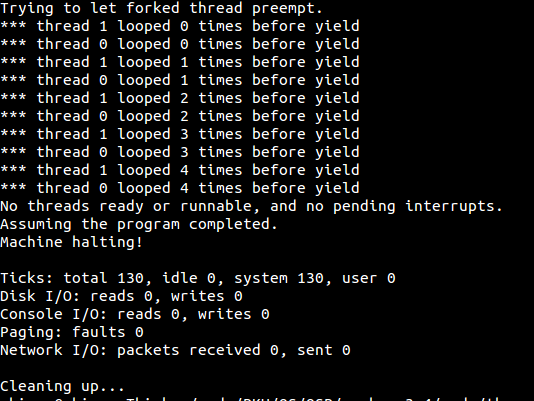
\includegraphics[width=3in]{ex22.png}
\end{figure}

我们看到由于fork线程的优先级被提高了。所以先优先进行fork线程,抢占式的效果就出来了。

新加几个线程并简单改写threadtest如下:
\begin{lstlisting}
void ThreadTest3() {
    printf("Creating thread 1\n");
    Thread *t1 = new Thread("forked 1 with 7", 8);
    t1->Fork(LongThread, 1);
    printf("Creating thread 2\n");
    Thread *t2 = new Thread("forked 2 with 8", 9);
    t2->Fork(SimpleThread, 2);
    printf("Creating thread 3\n");
    Thread *t3 = new Thread("forked 3 with 5", 7);
    t3->Fork(SimpleThread, 3);
    printf("Creating thread 4\n");
    Thread *t4 = new Thread("forked 4 with 2", 5);
    t4->Fork(SimpleThread, 4);
    printf("Creating thread 5\n");
    Thread *t5 = new Thread("forked 5 with 3", 6);
    t5->Fork(SimpleThread, 5);
}

void
SimpleThread(int which)
{
    int num;
    
    for (num = 0; num < 1; num++) {
	printf("*** thread %d looped %d times before yield\n", which, num);
       currentThread->Yield();
	printf("*** thread %d looped %d times after yield\n", which, num);
    }
}
\end{lstlisting}

结果如下:
\begin{figure}[h]
 \centering
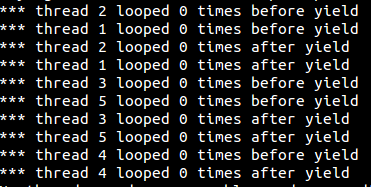
\includegraphics[width=3in]{ex23.png}
\end{figure}

我们可以看到这样的结果就是根据优先级两个高优先级的程序会相互交替执行。仔细分析我们会发现这种情况就是基于优先级的抢占式调度算法的普遍情况。

\subsection*{Exercise 4}
\textbf{增加全局线程管理机制}\\
我由拓展设计了两个不同的调度算法,分别是时间片轮转和简单CFS的调度算法。实现这两个算法主要的涉及点是:
\begin{itemize}
\item 对于RR算法,我们只需要初始化一个timer并激活YieldOnReturn即可。这一点可以和原来的rs模式复用。
\item 对于CFS,我们可以做一下简化。每次调度运行priority个周周期,并且vruntime+1,就绪队列根据vruntime进行排序。为thread设计一个getKey接口后,CFS就可以和基于优先级的抢占式算法复用优先级接口。
\end{itemize}
我用一个全局变量来区分调度算法,由命令行参数决定。
由于之前提到的yieldOnReturn机制,所以我们对代码的改写只需要在yield中进行即可。

修改后的主要代码如下:
\begin{lstlisting} 
Thread::Thread(char* threadName, int _priority, int _uid)
{
	...
    if(!strcmp(name, "main")) {
        priority = 11;
    }
    lastTick = currentTick = 0;
    if(sch_mode == 'l') {
        tickStep = priority;
    } else {
        tickStep = 1;
    }
}

int Thread::getKey() {
    if(sch_mode == 'r' || sch_mode == 'f') return 0;
    if(sch_mode == 'p') return -priority;
    if(sch_mode == 'l') {
        return (currentTick / priority);
    }
}

void
Thread::Yield ()
{
	...    
    /** Added **/
    bool change = false;
    TS();
    currentTick++;
    if(currentTick - lastTick == tickStep) {
        lastTick = currentTick;
        change = true;
    } else {
        change = false;
    }
    if(sch_mode == 'f' || sch_mode == 'p') {
        change = true;
    }
    DEBUG('t', "Cur, Lst = %d %d\n", currentTick, lastTick);
    if(change) {
        nextThread = scheduler->FindNextToRun();
        if (nextThread != NULL) {
        scheduler->ReadyToRun(this);
        scheduler->Run(nextThread);
        }
    } else {
        scheduler->Run(this);
    }
    DEBUG('t', "Before SET");
    (void) interrupt->SetLevel(oldLevel);
    DEBUG('t', "End Yielding");
}

void
Scheduler::ReadyToRun (Thread *thread)
{
    DEBUG('t', "Putting thread %s on ready list.\n", thread->getName());

    thread->setStatus(READY);
    readyList->SortedInsert((void *)thread, thread->getKey());
}


\end{lstlisting}

这里有个小trick,就是对yield的理解。yield主要功能是主动让出CPU,但是这个功能是留给用户的还是留给系统的有待斟酌。我的理解是后者,这个yield并不是sleep,不应该由用户发起,所以yield的主要作用就应该是留给系统在调度中使用的。所以在threadtest中我并没有插入yield。我的第一个threadtest如下设计:

我的测试threadtest如下设计:
\begin{lstlisting}
void ThreadTest3() {
    printf("Creating thread 1\n");
    Thread *t1 = new Thread("forked 1 with 7", 8);
    t1->Fork(LongThread, 1);
    printf("Creating thread 2\n");
    Thread *t2 = new Thread("forked 2 with 8", 9);
    t2->Fork(LongThread, 2);
    printf("Creating thread 3\n");
    Thread *t3 = new Thread("forked 3 with 5", 7);
    t3->Fork(LongThread, 3);
    printf("Creating thread 4\n");
    Thread *t4 = new Thread("forked 4 with 2", 5);
    t4->Fork(LongThread, 4);
    printf("Creating thread 5\n");
    Thread *t5 = new Thread("forked 5 with 3", 6);
    t5->Fork(LongThread, 5);
}

void LongThread(int tid) {
    DEBUG('t', "begin %d\n", tid);
    while(currentThread->getCurrentTick() < 5) ;
    printf("Thread %d finished\n", tid);
    return;
}
\end{lstlisting}

结果是:\textbf{死机了!}

于是我打开各种调试信息,发现当一个线程进入while循环后就没有时钟中断发生了。我百思不得其解只能深入探索Nachos的中断机制。终于找到了原因所在,那就是时钟是由中断开关触发的(我觉得非常不合理)。

于是我在LongThread中加入了两句SetLevel,成功输出了。
RR的结果(加入了printf细节)是:
\begin{figure}[h]
 \centering
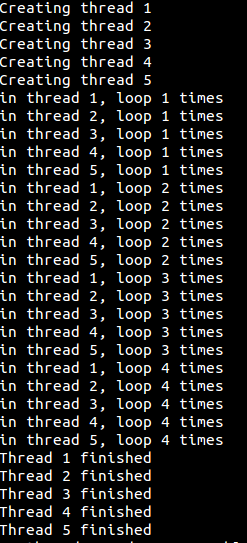
\includegraphics[width=2in]{ex24.png}
\end{figure}

可见轮转正常。RR不需要优先级,否则又是两个高优先级的轮着运行了。

CFS的结果(把结束判断的5改成了99)是:
\begin{figure}[h!]
 \centering
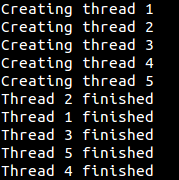
\includegraphics[width=1.5in]{ex25.png}
\end{figure}

可见高优先级的线程的确是最先结束的。这里由于篇幅限制我省略了详细的printf输出,不过输出表示整个运转是正常的。

\subsection*{各调度算法总结}
\begin{table}[h]
\centering
\footnotesize
\begin{tabular}{|c|c|c|c|c|}\hline
& \textbf{FIFO} & \textbf{Preempt} & \textbf{RoundRobin} & \textbf{CFS} \\\hline
\textbf{命令行参数} & f & p & r & l \\\hline
\textbf{排序键值} & 无 & priority & 无 & currentTick/priority \\\hline
\textbf{是否触发时间片} & N & N & Y & Y \\\hline
\end{tabular}
\end{table}


\section{遇到的困难以及解决办法}
\subsection*{底层代码}
之前助教也提到过,Nachos是建立在虚拟机上的,所以和一个真实操作系统还是有所差距的。尤其到了底层代码上,虚拟机并不直接操作硬件,所以理解上我也碰到了一些问题。其中最主要的就是对Nachos中断机制。之前也提到了,我在Nachos的时钟上卡了好久,这也是我在整个代码设计中最大的困难了。
\subsection*{参数调整和测试设计}
由于不同的参数导致的结果会有不同,所以到底选择哪些参数比较好还是需要斟酌一下的。我最后选择的TimerSlice是20,用户线程的优先级是1-10,main线程的优先级是11。由于这些参数主要是宏定义,所以修改起来比较简单,但调试和测试的过程是比较麻烦的。
\subsection*{调度算法的细节理解}
虽然在操作系统课上我们学过了很多的调度算法,也对调度算法有了一个比较全面的了解。但是这种了解到了实习课上还是远远不够的。由于涉及的代码更底层,所以我们还需要对每个算法细节又理解。需要深入理解readylist上个进程的具体执行顺序,以及各种操作都会触发调度算法的哪些行为。还是有一些预备知识需要积累的。
\subsection*{各算法的整合}
另外一个需要考虑的就是整个nachos上每个调度算法的横向兼容性。在我的代码里,这些算法的决定是由命令行参数决定的。我为nachos设计了一个全局变量schmode来标识使用的调度算法。我觉得这样的设计是最符合常规的。

\section{收获与感想}
总的来说,这次的lab还算是一个比较复杂的lab。需要设计的代码量比较大,也需要比较仔细地去分析。与此同时由于更接近底层,所以调试时间也比较长。我还是花了不少时间在这个lab上的。

不过虽然复杂,但是由于其涉及的内容仅仅是调度算法,所以问题的广度不算太大。如果在设计之前对每个调度算法先进行简单的调研以及思考,代码设计的整个过程也还是比较清晰的。

当然,虽然我整合了四个调度算法,但是都只是进行了简单的实现。效率也暂时没有进行深入评测。如果再给我写一次,或许我会深入钻研一种调度算法并进行一些高效的优化。

\section{意见与建议}
无。

\section{参考资料}
\begin{itemize}
\item 《现代操作系统》
\item 《Linux内核设计与实现》
\end{itemize}

\end{document}